%  LaTeX support: latex@mdpi.com 
%  In case you need support, please attach all files that are necessary for compiling as well as the log file, and specify the details of your LaTeX setup (which operating system and LaTeX version / tools you are using).

%=================================================================
\documentclass[applsci,article,preprint,moreauthors,pdftex]{Definitions/mdpi} 

% If you would like to post an early version of this manuscript as a preprint, you may use preprint as the journal and change 'submit' to 'accept'. The document class line would be, e.g., \documentclass[preprints,article,accept,moreauthors,pdftex]{mdpi}. This is especially recommended for submission to arXiv, where line numbers should be removed before posting. For preprints.org, the editorial staff will make this change immediately prior to posting.

%--------------------
% Class Options:
%--------------------
%----------
% journal
%----------
% Choose between the following MDPI journals:
% acoustics, actuators, addictions, admsci, aerospace, agriculture, agriengineering, agronomy, algorithms, animals, antibiotics, antibodies, antioxidants, applsci, arts, asc, asi, atmosphere, atoms, axioms, batteries, bdcc, behavsci , beverages, bioengineering, biology, biomedicines, biomimetics, biomolecules, biosensors, brainsci , buildings, cancers, carbon , catalysts, cells, ceramics, challenges, chemengineering, chemistry, chemosensors, children, cleantechnol, climate, clockssleep, cmd, coatings, colloids, computation, computers, condensedmatter, cosmetics, cryptography, crystals, dairy, data, dentistry, designs , diagnostics, diseases, diversity, drones, econometrics, economies, education, ejihpe, electrochem, electronics, energies, entropy, environments, epigenomes, est, fermentation, fibers, fire, fishes, fluids, foods, forecasting, forests, fractalfract, futureinternet, futurephys, galaxies, games, gastrointestdisord, gels, genealogy, genes, geohazards, geosciences, geriatrics, hazardousmatters, healthcare, heritage, highthroughput, horticulturae, humanities, hydrology, ijerph, ijfs, ijgi, ijms, ijns, ijtpp, informatics, information, infrastructures, inorganics, insects, instruments, inventions, iot, j, jcdd, jcm, jcp, jcs, jdb, jfb, jfmk, jimaging, jintelligence, jlpea, jmmp, jmse, jnt, jof, joitmc, jpm, jrfm, jsan, land, languages, laws, life, literature, logistics, lubricants, machines, magnetochemistry, make, marinedrugs, materials, mathematics, mca, medicina, medicines, medsci, membranes, metabolites, metals, microarrays, micromachines, microorganisms, minerals, modelling, molbank, molecules, mps, mti, nanomaterials, ncrna, neuroglia, nitrogen, notspecified, nutrients, ohbm, optics, particles, pathogens, pharmaceuticals, pharmaceutics, pharmacy, philosophies, photonics, physics, plants, plasma, polymers, polysaccharides, preprints , proceedings, processes, proteomes, psych, publications, quantumrep, quaternary, qubs, reactions, recycling, religions, remotesensing, reports, resources, risks, robotics, safety, sci, scipharm, sensors, separations, sexes, signals, sinusitis, smartcities, sna, societies, socsci, soilsystems, sports, standards, stats, surfaces, surgeries, sustainability, symmetry, systems, technologies, test, toxics, toxins, tropicalmed, universe, urbansci, vaccines, vehicles, vetsci, vibration, viruses, vision, water, wem, wevj

%---------
% article
%---------
% The default type of manuscript is "article", but can be replaced by: 
% abstract, addendum, article, benchmark, book, bookreview, briefreport, casereport, changes, comment, commentary, communication, conceptpaper, conferenceproceedings, correction, conferencereport, expressionofconcern, extendedabstract, meetingreport, creative, datadescriptor, discussion, editorial, essay, erratum, hypothesis, interestingimages, letter, meetingreport, newbookreceived, obituary, opinion, projectreport, reply, retraction, review, perspective, protocol, shortnote, supfile, technicalnote, viewpoint
% supfile = supplementary materials

%----------
% submit
%----------
% The class option "submit" will be changed to "accept" by the Editorial Office when the paper is accepted. This will only make changes to the frontpage (e.g., the logo of the journal will get visible), the headings, and the copyright information. Also, line numbering will be removed. Journal info and pagination for accepted papers will also be assigned by the Editorial Office.

%------------------
% moreauthors
%------------------
% If there is only one author the class option oneauthor should be used. Otherwise use the class option moreauthors.

%---------
% pdftex
%---------
% The option pdftex is for use with pdfLaTeX. If eps figures are used, remove the option pdftex and use LaTeX and dvi2pdf.

%=================================================================
\firstpage{1}  
\makeatletter 
\setcounter{page}{\@firstpage} 
\makeatother
\pubvolume{xx}
\issuenum{1}
\articlenumber{5}
\pubyear{2019}
\copyrightyear{2019}
%\externaleditor{Academic Editor: name}
\history{Received: date; Accepted: date; Published: date}
%\updates{yes} % If there is an update available, un-comment this line

%% MDPI internal command: uncomment if new journal that already uses continuous page numbers 
%\continuouspages{yes}

%------------------------------------------------------------------
% The following line should be uncommented if the LaTeX file is uploaded to arXiv.org
%\pdfoutput=1

%=================================================================
% Add packages and commands here. The following packages are loaded in our class file: fontenc, calc, indentfirst, fancyhdr, graphicx, lastpage, ifthen, lineno, float, amsmath, setspace, enumitem, mathpazo, booktabs, titlesec, etoolbox, amsthm, hyphenat, natbib, hyperref, footmisc, geometry, caption, url, mdframed, tabto, soul, multirow, microtype, tikz

\usepackage{mathptmx}       % selects Times Roman as basic font
\usepackage{helvet}         % selects Helvetica as sans-serif font
\usepackage{courier}        % selects Courier as typewriter font
\usepackage{type1cm}        % activate if the above 3 fonts are
                            % not available on your system
%
\usepackage{amsmath}

\newtheorem*{problem}{Problem}

\usepackage{makeidx}         % allows index generation
\usepackage{graphicx}        % standard LaTeX graphics tool
                             % when including figure files
\usepackage{multicol}        % used for the two-column index
\usepackage{blindtext}
\newenvironment{thisnote}{\par\color{blue}}{\par}
%=================================================================
%% Please use the following mathematics environments: Theorem, Lemma, Corollary, Proposition, Characterization, Property, Problem, Example, ExamplesandDefinitions, Hypothesis, Remark, Definition, Notation, Assumption
%% For proofs, please use the proof environment (the amsthm package is loaded by the MDPI class).
\newtheorem{df}{Definition}

%=================================================================
% Full title of the paper (Capitalized)
\Title{A diagnostics of conveyor belt splices}

%Using genetic algorithms for diagnostics of conveyor belts


% Author Orchid ID: enter ID or remove command
\newcommand{\orcidauthorA}{0000-0002-3019-9773} % Add \orcidA{} behind the author's name
\newcommand{\orcidauthorB}{0000-0003-1297-3590} % Add \orcidA{} behind the author's name
\newcommand{\orcidauthorC}{0000-0003-4781-9972} % Add \orcidB{} behind the author's name
\newcommand{\orcidauthorD}{0000-0002-8802-9865} % Add \orcidA{} behind the author's name
\newcommand{\orcidauthorE}{0000-0002-6565-203X} % Add \orcidA{} behind the author's name

% Authors, for the paper (add full first names)
\Author{Tomasz Koz{\l}owski$^{1,*}$\orcidA{}, and Jacek Wodecki$^{2}$\orcidB{}, and Rados{\l}aw Zimroz$^{2}$\orcidC{}, and Ryszard B{\l}a{ż}ej$^{2}$\orcidD{}, and Monika Hardyg{\'o}ra$^{2}$\orcidE{}}

% Authors, for metadata in PDF
\AuthorNames{Tomasz Koz{\l}owski and Jacek Wodecki and Rados{\l}aw Zimroz and Ryszard B{\l}ażej and Monika Hardygóra}

% Affiliations / Addresses (Add [1] after \address if there is only one affiliation.)
\address{%
$^{1}$ \quad Faculty of Electronics, Wroclaw University of Science and Technology, Janiszewskiego 11/17, 50-372 Wroclaw, Poland; t.kozlowski@pwr.edu.pl\\
$^{2}$ \quad Faculty of Geoengineering, Mining and Geology, Wroclaw University of Science and Technology, Na Grobli 15, 50-421 Wroclaw, Poland; \{jacek.wodecki, radoslaw.zimroz, ryszard.blazej, monika.hardygora\}@pwr.edu.pl
}

% Contact information of the corresponding author
\corres{Correspondence: t.kozlowski@pwr.edu.pl}

% The commands \thirdnote{} till \eighthnote{} are available for further notes

%\simplesumm{} % Simple summary

%\conference{} % An extended version of a conference paper

% Abstract (Do not insert blank lines, i.e. \\) 
\abstract{
Damage detection in complex mechanical structures is important for cost-effective and safe operation. Conveyor belt with steel cords is used for bulk material transport in mining companies. Due to harsh environmental conditions, both covers and cords are subjected to damages. As lengths of conveyors may vary from dozen of meters to kilometers, a belt loop consists of many connected belt pieces. So, the condition of splices between belt pieces is also critical. For both steel cords damage/wear detection and splices condition evaluation the NDT techniques based on magnetic field measurement and variability analysis are used. To obtain appropriate resolution multi-channel data is collected. Here we propose a pre-processing technique developed for signal synchronization for biased splices data. The biased splices mean a phase shift between signals from a multi-channel sensor due to the design technology of the splice. As the quality of the splice is related to the appropriate precision of splice production, splice evaluation is defined as a similarity analysis of each signal with respect to the estimated pattern. Due to the mentioned phase shift, signals should be "synchronized" first, before final analysis. In industrial conditions, many factors may influence the signal shape. Thus, the problem of automated synchronization by shifting the signals may be defined as a multidimensional optimization problem. Here, we proposed to use a Genetic Algorithm with an algorithmically simple cost function for that purpose. In this paper, the authors propose an automated procedure applied to real measurement data and final results. A multidimensional optimization has been compared to simple signal shifting according to several criteria and GA-based results appeared as the best one.
}
%\\The paper discusses the synchronization of magnetic signals obtained from the splices of steel-cord conveyor belts. The synchronization of functions from multiple channels is a problem of bias splices. Moreover, signals from bias splices are similar to signals from straight splices. So hence the same methods can be used for both types. Synchronization accuracy has an impact on the accuracy of subsequent estimation of splice technical conditions. Synchronization was performed using three methods: manual method, by single-point algorithm and genetic algorithm method. The paper describes in detail the advantages and disadvantages of every method, presents measurement results, and compares them. }

% Keywords
\keyword{conveyor belt, signal processing, genetic algorithm, NDT, defectoscopy}

\begin{document}

\section{Introduction}
Conveyor belts are used for transport in many industries, mainly: mining, logistics, civil engineering. From the very beginning various research related to optimization, energy efficiency or condition monitoring including magnetic monitoring of steel cord conveyor belts were initiated. Since then a number of solutions/systems were developed worldwide that allow optimization and non-invasive inspection of a whole conveyor \cite{8621649, Stefaniak_CMMNO2018, Carvalho2020, Mu2020, Yao2020, Zhang2020, Rudawska20201}, belt core \cite{harrison1985magnetic, kuzik1996scanning, yulin1999development, xiao2012electromagnetic, blazej2014high, fedorko2016possibilities}, drive units (gearbox, pulleys, bearings) \cite{Grzesiek2020,obuchowski2014recent,hebda2020selection,Wodecki201886}, idlers \cite{Molnar2020, Szrek2020, Liu20202689, Stehlikova2020, LIU2018277, krol_diagnostyka, krol_miningscience}. Recently inspection procedures started to be robotized \cite{zimrozMPES2019, Carvalho2020, Szrek2020}.

One of the most difficult components to diagnose is the conveyor belt. For belt with steel cords, magnetic field measurements have been proposed in 80s by Harrison \cite{harrison1985magnetic}. Magnetic field measurements are an accurate technique for testing ferromagnetic materials \cite{wang2012review}. Non-destructive testing using a magnetic phenomenon is a common method in detecting geometric discontinuities (damages) and fatigue states in materials. An example of using magnetic defectoscopy to assess the technical condition in machine elements are the cases of examination of train wheels \cite{le2013nondestructive}, pipes \cite{jarvis2016current}, wire ropes \cite{yan2017online}. The issue raised in this article are magnetic signals measured from steel cords in a conveyor belt.

Although there are some works on the diagnosis of belt with steel cord \cite{harrison1985magnetic,kuzik1996scanning,yulin1999development,xiao2012electromagnetic,blazej2014high,fedorko2016possibilities}, they are mainly concerned with detecting damage and evaluating technical condition of belt sections. Surprisingly, issues relating to the splices have been omitted. Splice technical condition may be evaluated during both regular service inspection of the belt as well as during production phase, as splice quality control. 

NDT-related processing of signals acquired from the belt one may face several important issues. First of all, to obtain the appropriate precision of damage detection, the multi-channel measurement system is used. As mentioned, it may be assumed that the average length of belt conveyors is 1 km. It gives a 2 km belt length and consequently, generates a lot of data to process. These data may be noisy as usual in a real industrial case. For example, the paper \cite{ma2016noise} deals with the issue of removing noise from electromagnetic signals coming from a conveyor belt with steel cords. 

From a signal processing point of view the task is to detect, extract and model (describe) disturbances in the signal related to splices i.e. places when two pieces of the belt are connected. It should be done for each sensor (each sensor array section, i.e. each part of the belt width) and depends on the design of the splice.

From a theoretical point of view, each signal (each belt width part) should be very similar for high-quality splices. If some errors have appeared during splice production, they will be sources of additional disturbances and they will influence the signal shape. Changes in signal shape may be also related to wear or fault that will rise during operation.

Practically, we would like to compare signals from all channels using some criteria. In case of biased splices, signals are phase-shifted as the beginning of the splice is shifted for each belt width section. For good condition splice - one may simply find a difference in phase of each signal with comparison to the selected reference channel. In case of damaged splice (or with poor quality), simple-shifting becomes a multidimensional optimization problem. The reason for this is that it will be hard to find one reference point in the reference signal. Incorrect synchronization may lead to wrong conclusions. To overcome it, we have proposed a Genetic Algorithm based procedure to optimize signals shifting. Criteria for optimization have been defined, too. The presented method has been applied for both damaged belt splices and good quality splices.

The paper is organized in the following way: section 2 present description of the multi-channel data acquisition system and provide some details about the experiment in the mine. Section 3 provides basic knowledge about belt splice design that is a basis to define the problem for signal processing (discussed in section 4). The developed procedure for multi-channel data processing is provided in section 5, while section 6 presents results and discussion regarding the comparison of methods and obtained results. Finally, the conclusions section ends the paper.

\section{HRDS measurement system}

High Resolution Diagnostic System (HRDS) is a unique solution developed at Wroclaw University of Science and Technology as an output of research project. It was designed for the magnetic testing of conveyor belts with steel cords. HRDS system is based on the modified EyeQ$^{TM}$ system from rEscan company. The effects of the work including the modification of the existing and available system mainly consisted of its expansion and increasing the measurement capabilities. The number of sensors was increased, which resulted in a six-fold increase in the resolution of the measuring system and the development of a mobile data acquisition device. The extension and measurement capabilities of the developed HRDS system are described in the article \cite{blazej2014diagnostics}.

\begin{figure}[ht!]
\centering
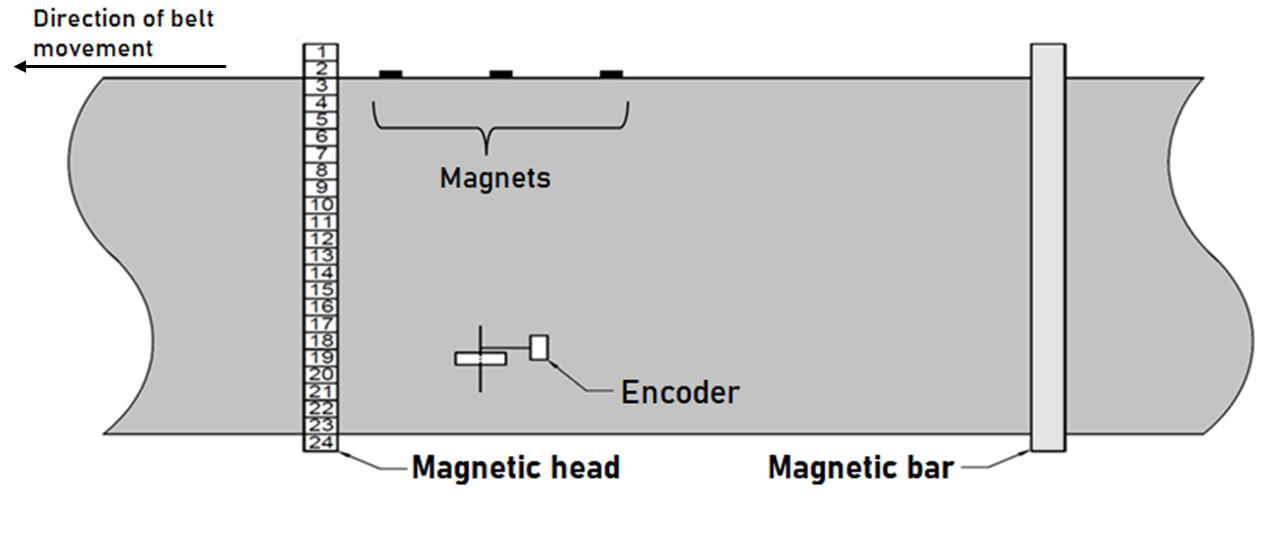
\includegraphics[width=.8\textwidth]{figs/hrds.png}
\caption{Scheme of the HRDS measuring system.}
\label{fig:hrds}
\end{figure}

\begin{figure}[ht!]
\centering
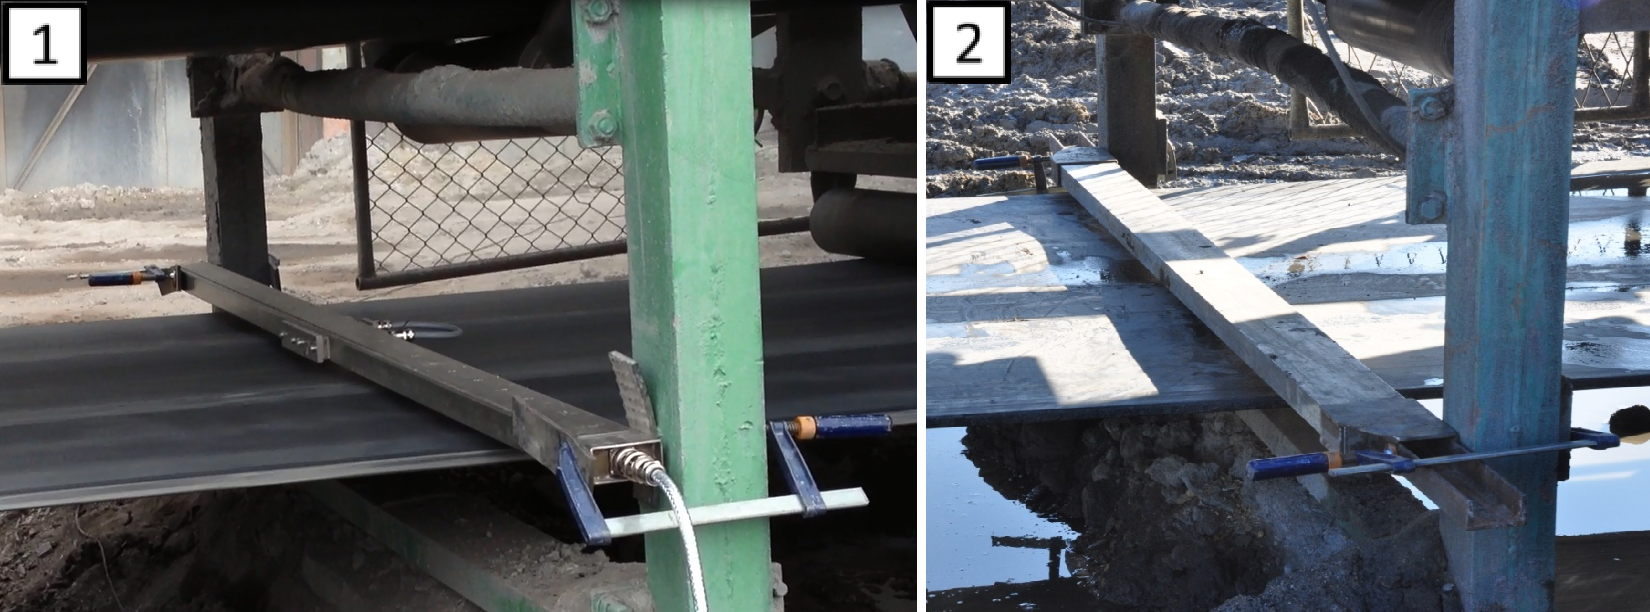
\includegraphics[width=\textwidth]{figs/hrds2.png}
\caption{Magnetic head (1) and magnetic bar (2) installed to belt conveyor construction.}
\label{fig:hrds2}
\end{figure}

The measurement method is based on the pre-magnetization of the steel cords in the core using a magnetic bar. The next step consists of the acquisition of the data from a magnetic head. In the magnetic head 24 coils with a resolution of 10 cm are located. This allows for testing on conveyor belts up to the width of 2,4 m with resolution of 0,1 m. The magnetic head and magnetic bar are placed perpendicular to the direction of belt movement. The coils (sensors) detect changes in the magnetic field generated by the magnetized steel cords located in the core of the conveyor belt. Magnetic field changes occur in the vicinity of damaged steel cords or splices. Scheme of the system  (Fig. \ref{fig:hrds}) and HRDS system during measurement have been presented in (Fig. \ref{fig:hrds2}-\ref{fig:hrds3}). The measurement system allows testing conveyor belts with speed of up to 10 m/s.

\begin{figure}[ht!]
\centering
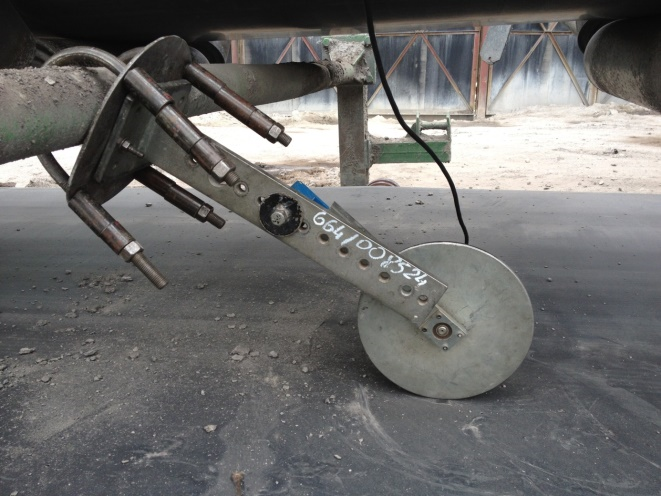
\includegraphics[width=.7\textwidth]{figs/hrds3.png}
\caption{Encoder installed to belt conveyor construction.}
\label{fig:hrds3}
\end{figure}

Also, several small neodymium magnets are attached to the periphery of the conveyor belt. The magnets are positioned 8-12 m apart to automatically identify full runs of the belt loop and thus the beginning and end of the belt loop. The magnets should not be attached in the area of the splices. The amplitude of the signal in the splice area distorts the reading of the signal generated by the neodymium magnets. Likewise, the sections where the magnets are attached to the belt can be marked. It allows to quickly find the magnets and remove them after the measurement (Fig. \ref{fig:hrds4}).

\begin{figure}[ht!]
\centering
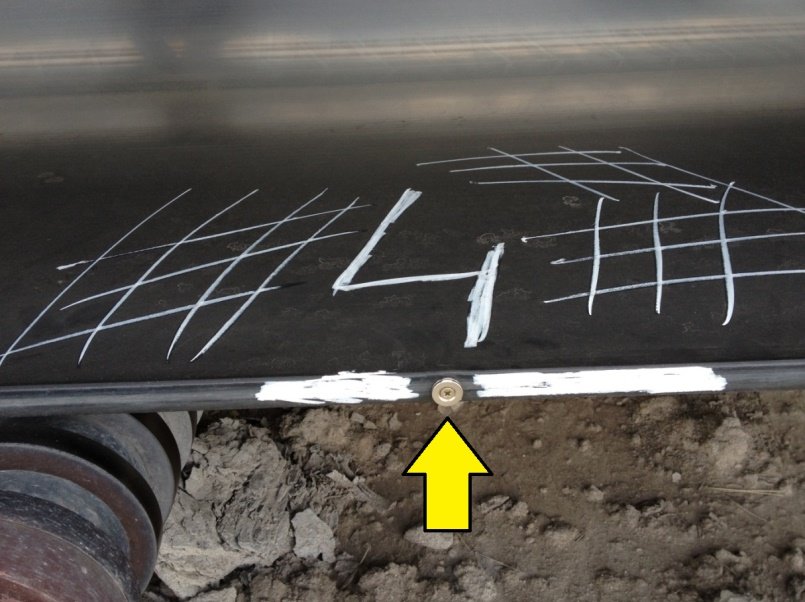
\includegraphics[width=.6\textwidth]{figs/hrds4.png}
\caption{One of the marked neodymium magnets attached to the conveyor belt.}
\label{fig:hrds4}
\end{figure}

The HRDS system data acquisition module is built into the Peli box. It consists of a signal recording module (CompactDAQ) and a portable tablet (Durabook) with an application (Fig. \ref{fig:hrds5}). After performing the measurement, it is possible to copy the data directly from the tablet to the computer, which allows for further analysis.

\begin{figure}[ht!]
\centering
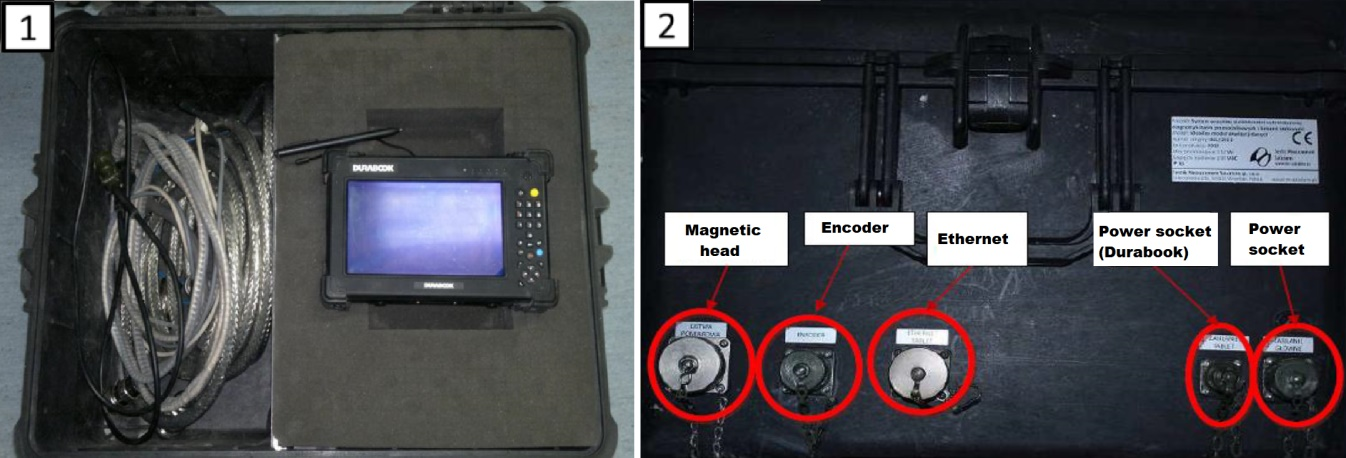
\includegraphics[width=\textwidth]{figs/hrds5.png}
\caption{HRDS system data acquisition module: Durabook tablet and CompactDAQ (1), plugs installed in the box (2).}
\label{fig:hrds5}
\end{figure}

\section{Conveyor belt splices}

As mentioned, due to the length of a conveyor, weight and size of the required belt it is not possible to use one piece of a belt, so it is divided into sections (100-400m) and these pieces are "reconnected" by adhesive, mechanical joints or vulcanization depending on belt type. These parts of the belt loop are by definition the weakest parts and thus evaluation of their condition is so important, see Fig. \ref{fig:belt_splice}

\begin{figure}[ht!]
\centering
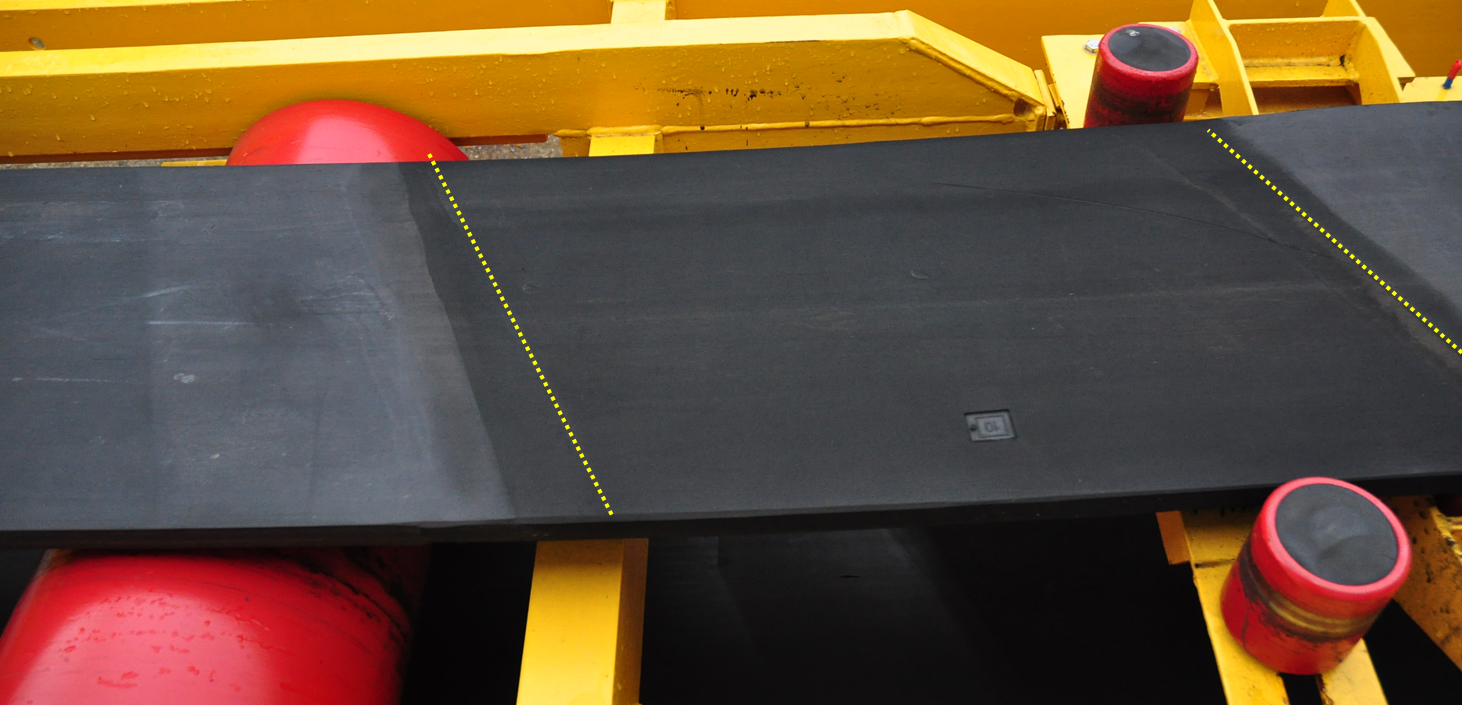
\includegraphics[width=\textwidth]{figs/splicetest.png}
\caption{Picture of the conveyor belt with splice}
\label{fig:belt_splice}
\end{figure}

In the case of conveyor belt splice, the change in the magnetic field is much greater than the change in the field due to the belt damage (see Fig. \ref{fig:belt_signal}). Unlike damage, the signal from the splice has a high amplitude across the entire width of the belt. This property was used to automatically detect splices in data from over the entire length of the belt.

\begin{figure}[ht!]
\centering
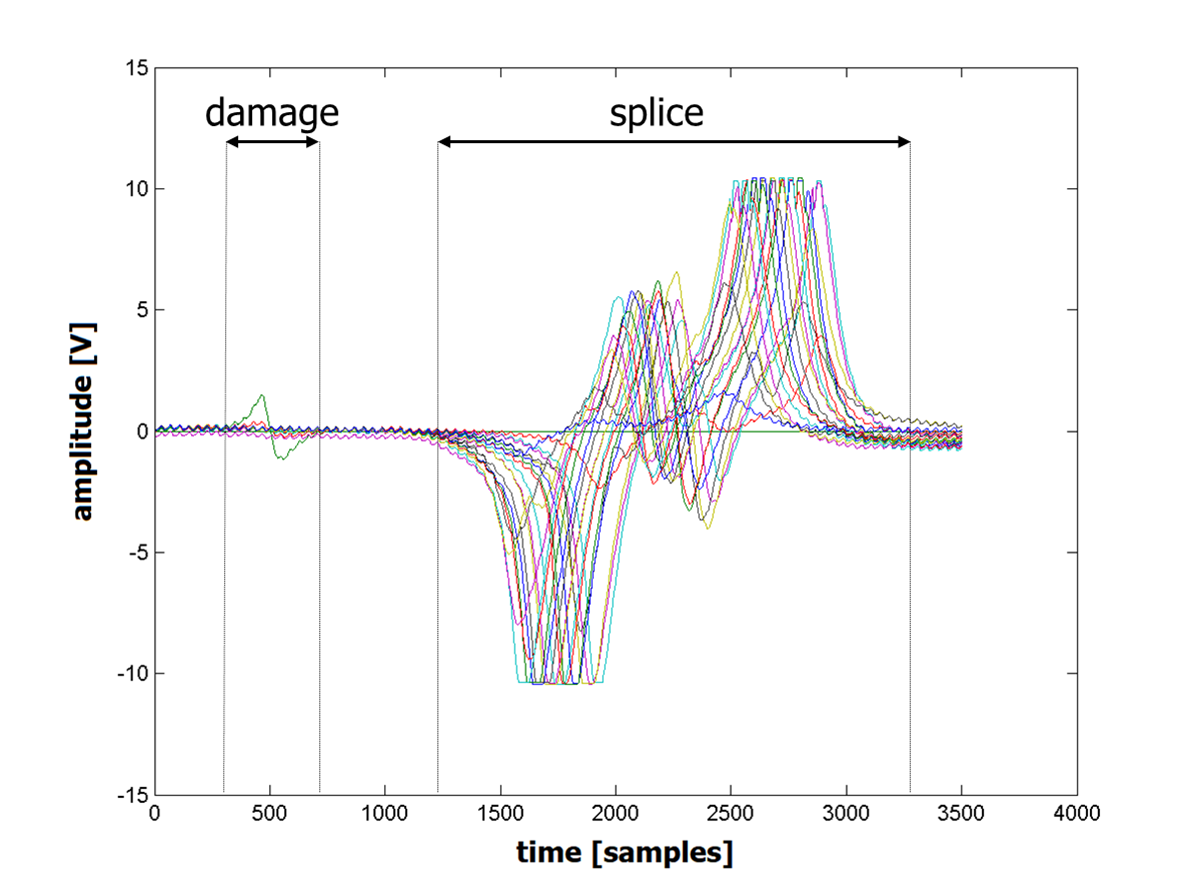
\includegraphics[width=.8\textwidth]{figs/splicedmg.png}
\caption{The raw magnetic field variations recorded for belt  with damage and splice}
\label{fig:belt_signal}
\end{figure}

The measurement data provides information on magnetic field variations across the belt’s length. This great amount of data requires initial classification. The first group comprises magnetic signals from belt sections, the second group comprises signals from splices. The algorithm described in \cite{blazej2013novel} included data from the first group. Splice is always the weakest part of conveyor belt. Splices were not analyzed due to the different characteristics of signals. The algorithm can save each splice to a separate file (Fig. \ref{fig:belt1}).

\begin{figure}[ht!]
\centering
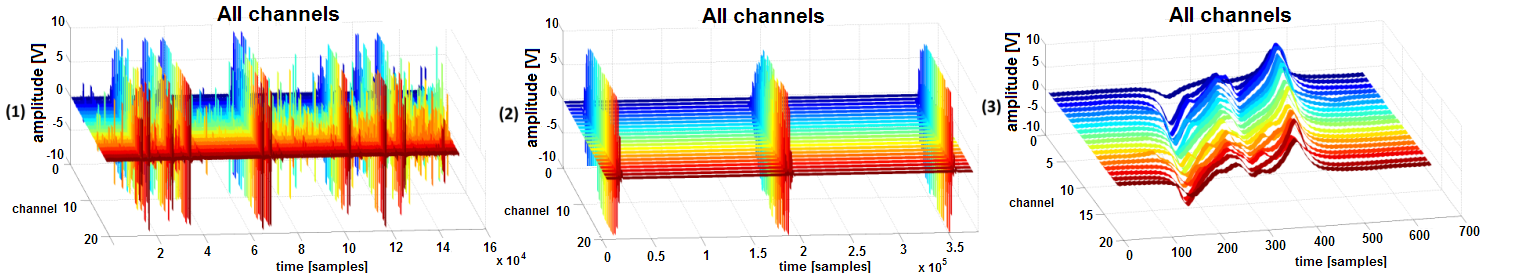
\includegraphics[width=\textwidth]{figs/belt1.png}
\caption{The magnetic field variations recorded for belt section with damages and splices (1), belt section only with splices (2), for a single splice (3).}
\label{fig:belt1}
\end{figure}

Unlike in the case of straight splices, the signals generated by bias splices are shifted in relation to each other as a function of time. Fig. \ref{fig:belt2} schematically shows signals characteristic for both splice types.

\begin{figure}[ht!]
\centering
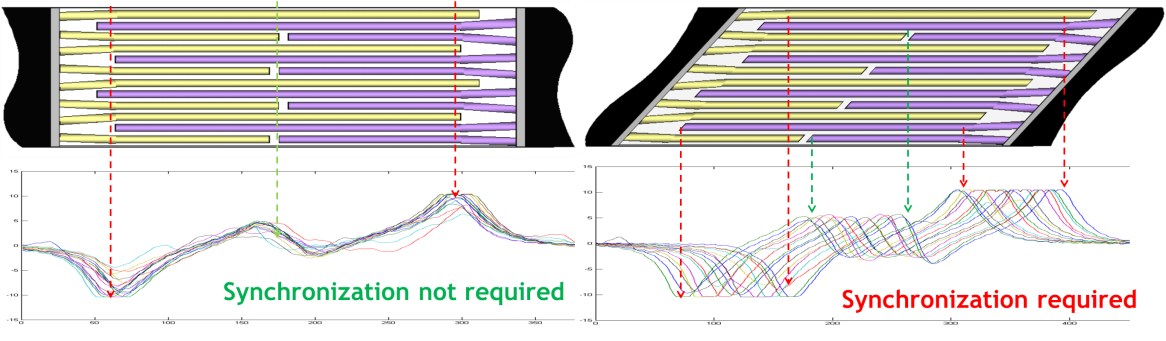
\includegraphics[width=\textwidth]{figs/belt2.png}
\caption{Signal characteristic for both splice types: straight splice (left) and bias splice (right).}
\label{fig:belt2}
\end{figure}

\section{Problem definition}

The analysis and comparison of signals from splices is problematic, as the signals are shifted with respect to each other. Shift values depend on splice geometry, production technology as well as wear processes. Note that shifts (nearly) do not occur in straight splices, which therefore cannot be compared with bias splices.

For good condition splice, each signal should have a similar shape, so just finding the phase difference and then shifting all signal with reference to the first channel may fix the problem. For bad conditions, it is very difficult to find a reference point and shifting the signal may provide misleading results. 

From an engineering perspective, the main goal is to shift each signal for bias splices by a certain value (with reference to selected signal) that would allow finding a minimum of their difference defined as simple sample-by-sample residual and RMS error. 
The ideal case means no difference between signals so RMSE will be zero.
For simple (not biased) splices, the shifting procedure is not required, one may simply compare signals as they are. It may be said that we developed a "synchronization" procedure for biased splices to convert them to "straight" splices and use a simple technique for splice condition evaluation.

From a practical point of view, the problem can be defined as finding the shift value for each channel, such that some predefined objective function describing error in mutual positioning of all channels is minimized. In the past, several attempts have been made to solve this problem either manually or using simple deterministic algorithms (also presented in this paper for reference). However, the authors propose to define the problem as an optimization problem. We consider the Genetic Algorithm (GA) as a potential tool, because of its ease of implementation and problem definition in such a case. GA is also very robust in avoiding local minima due to intrinsic solutions such as random mutation.

\section{Methodology}

Synchronization was performed using three methods: manual method, single-point method and genetic algorithm method, which is the selling point of this paper. Authors considered other methods that would allow to automatically synchronize the channels, however, they turned out to be infeasible in the realistic scenario.

The first considered method assumes using relative cross-correlation of the channels to detect shifts between them. It seems very straightforward and robust, however, edge channels with signal shapes, dissimilar to the rest, were in practice too irregular to be able to properly detect the shift for them. For this reason, it cannot be used, because there is a need to synchronize all the channels and not disregard the edge ones. For poor-quality splices, this method was completely unusable because cross-correlation did not allow to reliably detect the relative shifts because of too irregular shapes of the channels.

The second considered method assumes using a neural network to estimate the values of relative shifts. While theoretically possible, it would require a large dataset for learning. In such set parts of the signal containing information about the splices would need to be perfectly segmented, parameterized and labeled, which is practically impossible (another large-scale automated method would be needed to do that), but most importantly, it is infeasible because even within a single belt the splices can be so different that common parameterization, even if possible, would be meaningless, especially for automatic pre-labeling.

For those and other reasons, the authors decided to use a well-known, easy to set up optimization technique which is a genetic algorithm. The description of the methods and their results are presented below.

\subsection{Manual method}

The first method consisted in manually matching all signals from a single splice.  The method was based on the following algorithm (Fig. \ref{fig:block1}).

\begin{figure}[ht!]
\centering

\includegraphics[width=0.7\textwidth]{figs/block1.png}
\caption{Manual method synchronization algorithm.}
\label{fig:block1}
\end{figure}

The above algorithm assumes that initial shift values may not be satisfying to the user and allows to modify them repeatedly. Fig. \ref{fig:manual1} shows the first three steps of the algorithm: (1) loading two channels; (2) shifting the second channel in relation to the first channel; (3) loading the third channel, etc.

\begin{figure}[ht!]
\centering
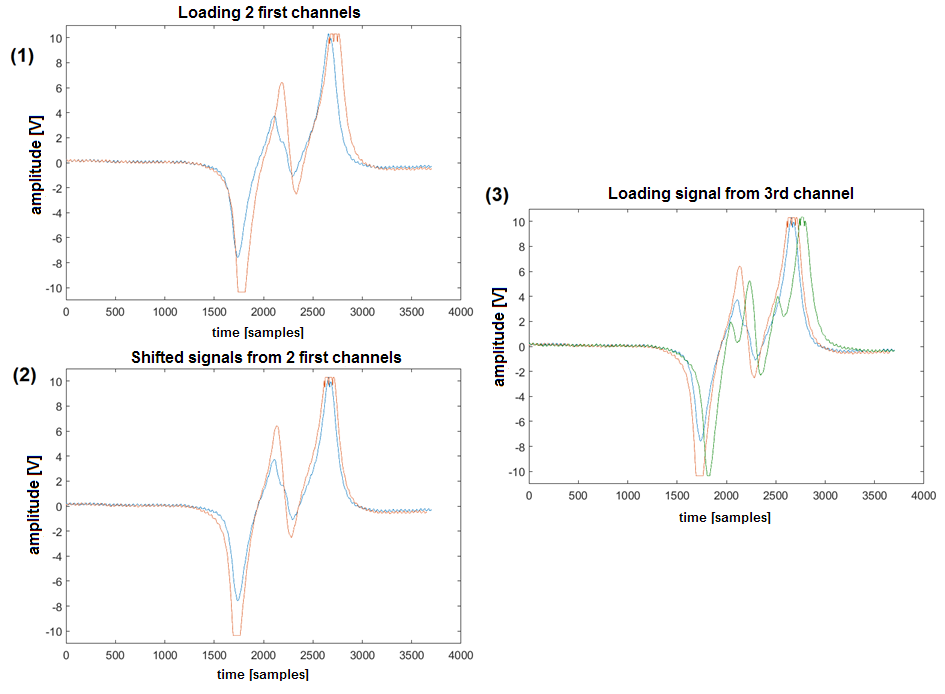
\includegraphics[width=0.9\textwidth]{figs/manual1.png}
\caption{First three steps presented for manual channel synchronization.}
\label{fig:manual1}
\end{figure}

As the above method is very time-consuming and provides results that depend on the user’s experience, automated synchronization methods are required to speed up the process. The disadvantages of the method make it impractical and hence this solution was not included in the comparison of the remaining methods discussed in chapter: comparison of algorithms. The method cannot be used in the mine, where the number of belt conveyors (and hence splices) makes it highly ineffective.

\subsection{Single-point algorithm}

Manual synchronization of one splice is time-consuming and inaccurate. This fact necessitated another method for signal matching. It was assumed that all signals (from one splice) should have uniform length (Fig. \ref{fig:block2}). Matching was performed for both correctly made and faulty splices (Fig. \ref{fig:fp1}).

\begin{figure}[ht!]
\centering

\includegraphics[width=0.65\textwidth]{figs/block2.png}
\caption{Single-point synchronization algorithm.}
\label{fig:block2}
\end{figure}

The results of using single-point algorithm were not satisfactory. In case of a faulty splice the differences between the lengths of particular signals were much greater that in case of a correctly made splice. The algorithm that synchronizes signals in relation to a single-point can be run within just a few seconds. This allowed for significant time savings as compared to the first method.

\begin{figure}[ht!]
\centering
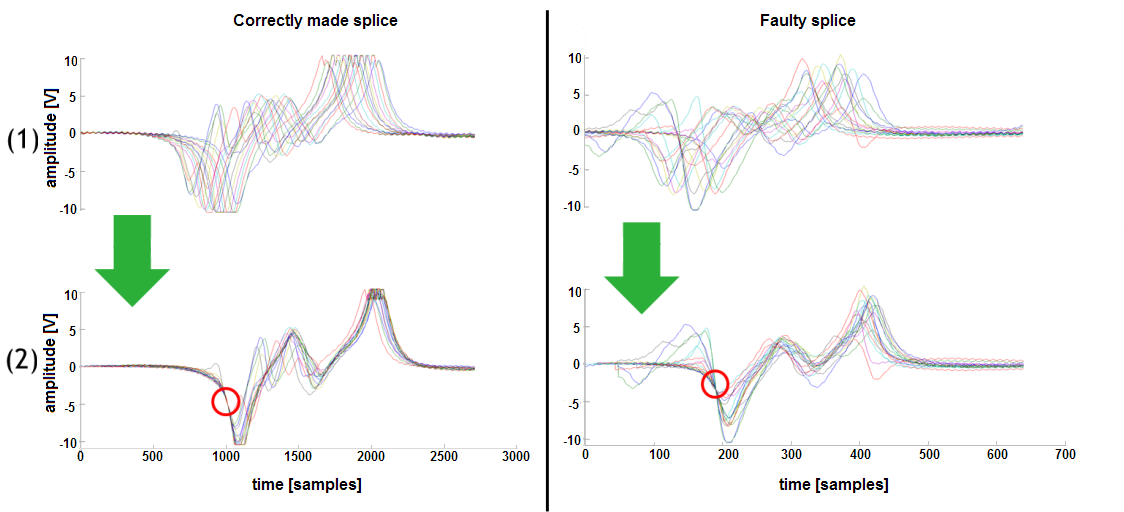
\includegraphics[width=\textwidth]{figs/fp1.png}
\caption{The results of synchronization performed with single-point algorithm for correctly made splice (on the left) and for faulty splice (on the right) with synchronization point marked (red circle).}
\label{fig:fp1}
\end{figure}

\subsection{Genetic algorithm}

Genetic algorithm is a simulated process of evolution, that contains the main features seen in biology \cite{darwin2008origin}. From implementation point of view, GA is a metaheuristic optimization technique. This concept has been introduced by Bagley’s thesis \cite{bagley1967behavior} and then developed in large part by Holland \cite{holland1989induction,holland1992adaptation}. Typically optimization problems are given as follows:

\begin{problem}
    Find an $x_0\in \mathbf{X}$ such that $f$ is minimal in $x_0$, where $f:\mathbf{X}\rightarrow \mathbb{R}$ is an arbitrary real-valued function, i.e. $f(x_0)=\min_{x\in X}f(x)$.
\end{problem}

Sometimes it is very difficult to obtain strict global solution, so in practice we want to find values $x$ that minimize the objective function $f$. One can write down the elementary structure of GA as follows:

\textbf{Algorithm:}

\textit{Compute initial population $B_0$;}

\textbf{WHILE} \textit{stopping condition not fulfilled} \textbf{DO}

\textbf{BEGIN}

\textit{select individuals for reproduction;}

\textit{create offspring by crossing individuals;}

\textit{occasionally mutate some individuals;}

\textit{compute new generation;}

\textbf{END}
\\
The main loop of GA performs the transition from one generation to the next using four basic components:
\begin{itemize}
    \item \textbf{Selection:} Selection of individuals for reproduction with respect to their fitness defined with objective function.
    \item \textbf{Crossover:} Generation of offspring based on the information pulled from two individuals.
    \item \textbf{Mutation:} Random deformation of the chromosomes with a certain probability. This serves for generating genetic diversity and, as an effect, that local minima can be avoided.
    \item \textbf{Sampling:} Procedure which computes a new generation from the previous one and its offspring.
\end{itemize}

For the described application, GA is used to evolve the vector of 24 values corresponding to the shift of each channel to the right, expressed in samples. The number of total generations was set to 200, with a stall limit of 20 generations. Each population consisted of 450 individuals. The algorithm used the roulette method for the selection of individuals for reproduction and intermediate crossover function with a weight ratio equal to 0,8. Gene mutation probability was set to 0,01\%. The lower and upper bound for channel shift was defined as 1/6 of initial channel length. 

The fitness function is defined to be the sum of RMS errors between each channel in the current state of synchronization, and the median of all channels calculated at this state. This means that the more cohesively channels are synchronized, the lower the value of error. In fitness function, we use median instead of often used mean because it is less susceptible to outliers (i.e. edge channels that very often take a different shape than most) or to dissimilar shapes of individual channels (the worse splice quality the worse the mean value describes the trend across the channels in comparison to the median).

Results of the GA-based synchronization of channels are presented in Fig. \ref{fig:gen1}. Residual errors are low and channels are positioned very cohesively, especially for correctly made splices. Faulty splices are also synchronized very well, but it is more difficult to observe the synchronization quality just by looking at the result. The matrix of synchronized signals is not much longer than the original (about 15\% for correctly made splice, about 20\% for faulty splice).

\begin{figure}[ht!]
\centering
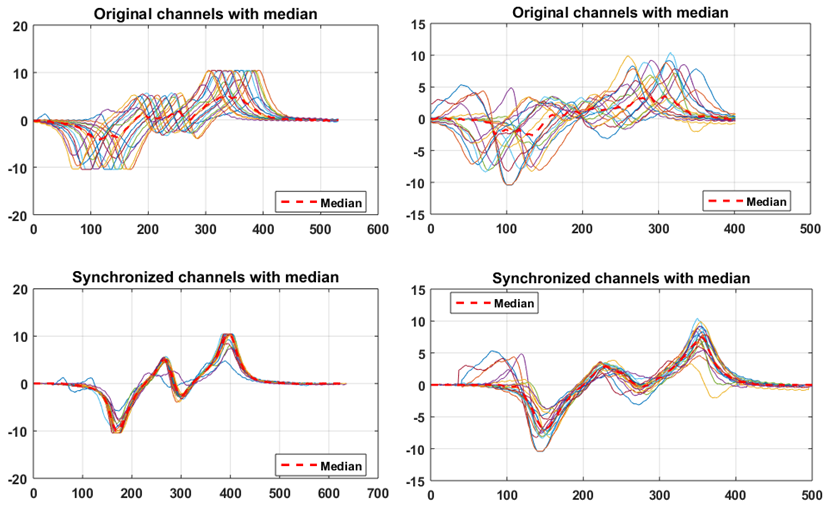
\includegraphics[width=\textwidth]{figs/gen1.png}
\caption{Results of synchronization with genetic algorithm for correctly made splice (left panels) and faulty splice (right panels).}
\label{fig:gen1}
\end{figure}

\section{Results and comparison of algorithms efficiency}

In this section we compare the performance of genetic algorithm and single-point algorithm. We disregard manual synchronization due to its impractical character, lack of repeatability and very long time of performing the task manually.

\subsection{Linearity criterion}

Linearity criterion works under the assumption that diagonal splices are manufactured with the linear shift, which translates into the idea that consecutive measurement channels should be shifted relative to each other by evenly spaced values (other words, each consecutive channel should be shifted by the linear function relative to the first channel). Results show that the genetic algorithm produces more linear shift than the single-point algorithm (Fig. \ref{fig:lin}, \ref{fig:lin2}). Besides visual evaluation, RMS error between the shift vector and its linear fit has been calculated (see Tab. \ref{tab:tab2}). 

\begin{table}[ht!]
    \centering
    \caption{RMS errors between shift vector and its linear approximation function.}
    \begin{tabular}{|l|l|l|l|}
    \hline
         & \textbf{Point} & \textbf{Genetic} & \textbf{Gain} \\ \hline
          \textbf{Correctly made splice} & 43 & 33 & ~30\% \\ \hline
          \textbf{Faulty splice} & 126 & 58 & ~117\% \\ 
    \hline
    \end{tabular}
    \label{tab:tab2}
\end{table}

The genetic algorithm outperforms single-point synchronization by far. In terms of linearity criterion, it performs about 30\% better for correctly made splice and about 117\% better for a faulty splice.

\begin{figure}[ht!]
\centering
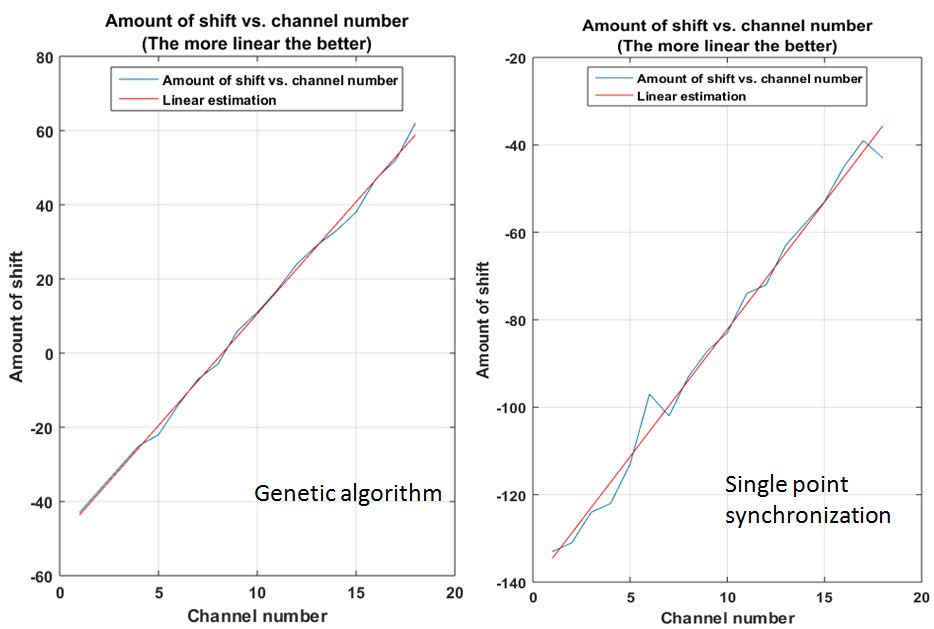
\includegraphics[width=0.8\textwidth]{figs/lin.png}
\caption{Linearity comparison for correctly made splice.}
\label{fig:lin}
\end{figure}

\begin{figure}[ht!]
\centering
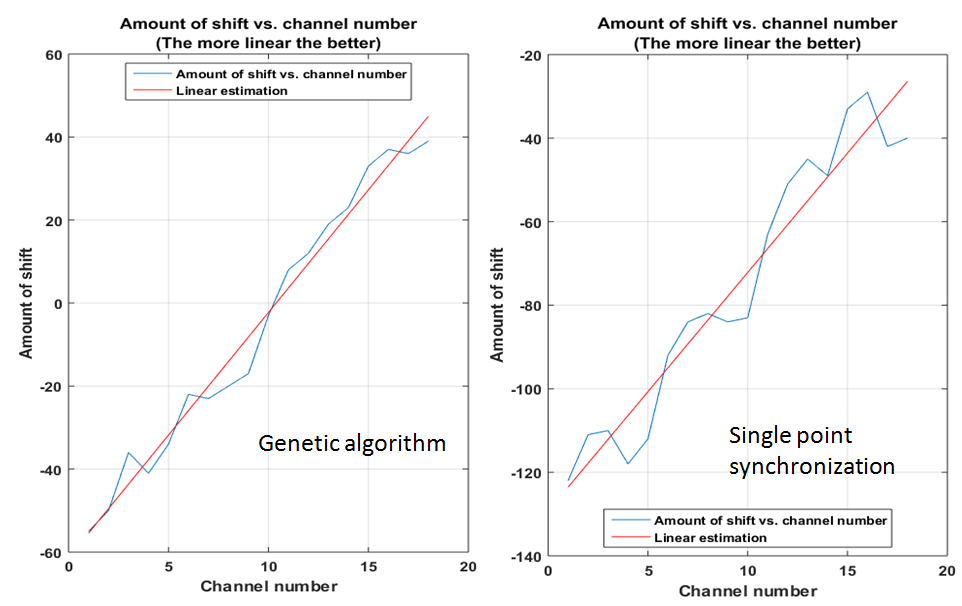
\includegraphics[width=0.8\textwidth]{figs/lin2.png}
\caption{Linearity comparison for faulty splice.}
\label{fig:lin2}
\end{figure}

\subsection{RMSE criterion}

This criterion is based on the measurement of RMS error between channels and median. Tab. \ref{tab:tab3} presents errors measured in both quality scenarios for the initial matrix of data, then for results of single-point synchronization and genetic algorithm.

\begin{table}[ht!]
    \centering
    \caption{RMS errors for initial data and results of synchronization with both algorithms.}
    \begin{tabular}{|l|l|l|l|l|}
    \hline
         & \textbf{Initial} & \textbf{Point} & \textbf{Genetic} & \textbf{Gain} \\ \hline
          \textbf{Correctly made splice} & 48,38 & 12,26 & 10,61 & ~15\% \\ \hline
          \textbf{Faulty splice} & 44,52 & 20,46 & 17,83 & ~15\% \\ 
    \hline
    \end{tabular}
    \label{tab:tab3}
\end{table}

Genetic algorithm again performs better, with a gain between single-point synchronization and genetic algorithm of about 15\%.

\subsection{Extension criterion}

In this case, we measure by how much-given algorithm has to extend the length of the initial data matrix. Each algorithm extends the matrix which is necessary to perform any shifting, but it is expected that the extension will be as small as possible. Tab. \ref{tab:tab4} shows the lengths of initial matrices along with final lengths after synchronization with both algorithms.

\begin{table}[ht!]
    \centering
    \caption{Lengths of initial data matrices and output matrices after synchronization.}
    \begin{tabular}{|l|l|l|l|l|}
    \hline
         & \textbf{Initial} & \textbf{Point} & \textbf{Genetic} & \textbf{Gain} \\ \hline
          \textbf{Correctly made splice} & 531 & 703 & 625 & ~12\% \\ \hline
          \textbf{Faulty splice} & 401 & 552 & 491 & ~12\% \\ 
    \hline
    \end{tabular}
    \label{tab:tab4}
\end{table}

Again, the genetic algorithm reveals better quality than single-point synchronization, with a gain of about 12\%.


%\end{thisnote}
\section{Conclusions}

Magnetic signals from conveyor belt bias splices were synchronized using the manual method, single-point method and genetic algorithm method. Each of the methods has been implemented in the Matlab software.
Manual synchronization is flawed with disadvantages and time consuming that disqualify it from comparison with the remaining algorithms.
Signal synchronization for total splice length was performed only in the case of the genetic algorithm. This fact was significant due to the differences between signal lengths for the same splice. The fitness function was set to be the sum of RMS errors between each channel and the median. This means that the more cohesively channels are synchronized, the lower the value of error.
Single-point algorithm and genetic algorithm were compared with each other using the criteria of linearity, RMSE and extension. The best results were obtained for the signals synchronized using the genetic algorithm and therefore this algorithm will be used in further research. In particular, GA was better than single-point method by 15\% using RMSE criterion, by 12\% using extension criterion, and even up to 117\% using linearity criterion. Signals synchronized using the genetic algorithm allow us to employ identical algorithms for inspecting the technical condition of both straight and bias splices, which significantly simplifies maintenance-related analytical procedures.


\section*{References}

\bibliography{mybibfile}

\end{document}

